% Agent-TTRL main paper (ACL 2027 framing; official ACL style files)
\documentclass[11pt]{article}
\usepackage[preprint]{acl}
\usepackage{times}
\usepackage{latexsym}
\usepackage{booktabs,amsmath,amssymb}
\usepackage{graphicx}
\title{Evidence-Gated Counterfactual Test-Time RL for Stateful Tool Agents}
\author{Anonymous}
\date{}
\begin{document}
\maketitle
% Abstract — Route B (v3 audit arc, 2026-08-26)
\begin{abstract}
Deployment-period parameter updates for tool-using agents (agent
test-time RL) are attractive, and recent systems report gains. We show
that the most common reported gains are artifacts of three silent
failure modes, demonstrated by re-running one pipeline under
increasingly strict protocol audits: (F1) \emph{served-policy drift} ---
the updated model never becomes the serving policy, so per-task
``update effects'' are sampling-stream displacement (96/96 identical
outcomes across arms); (F2) \emph{evaluator leakage and anchor
injection} --- the hidden evaluator controls episode termination and
hand-constructed anchors seed the replay buffer, producing a phantom
$+0.070$ AUPC transfer ($p{=}0.016$) that vanishes when both are
removed; (F3) \emph{protocol-correct updates are harmful} --- under
full isolation, REINFORCE-style updates significantly degrade
first-attempt AUPC (Mistral-7B: naive $-0.19$, $p{=}0.008$, 0/8 seeds
positive; frozen deterministic across seeds). The harm replicates on a
second backbone (Qwen2.5-7B: both update arms 8/8 seeds below frozen,
$p{=}0.008$), degrades the sealed never-trained holdout, and no
alternative update rule transfers. A pre-commit gate validating
candidate adapters on accessible evidence eliminates the harm (0/8
harmful commits). As a positive control, the same serving runtime
against the official \texttt{tau2} benchmark completes both evaluated
retail tasks with full reward in 5/10 seeded runs using only a local
14B model. We release the audit chain as a reproducible harness ---
policy-consistent runtime, request-scoped RNG, hidden-evaluator
isolation, accessible-evidence utilities, integration gates --- so any
agent test-time RL pipeline can be checked for these failure modes.
\end{abstract}

% Introduction — Route B (2026-08-25)
\section{Introduction}
Test-time reinforcement learning for language agents --- updating the
policy from the tasks it encounters during deployment so later tasks are
handled better --- has become a crowded and optimistic space. Systems
report gains on math reasoning~\cite{ttrl2025}, tool
use~\cite{t3rl2026}, instance-specific
refinement~\cite{staror2026}, and live in-episode updates with runtime
serving~\cite{att2026}. The deployment setting is genuinely important:
agents deployed in production receive partial, endogenous feedback and
cannot be retrained offline.

But the setting is also uniquely hard to evaluate honestly. Three
properties conspire:

\begin{itemize}
\item \textbf{Training and serving can silently diverge.} The model
  that receives the gradient may not be the model that generates the
  next first attempt. When they diverge, per-task differences between
  frozen and update arms are unidentifiable: they can come entirely
  from sampling-stream displacement --- update arms draw more random
  numbers --- rather than from policy change.
\item \textbf{The evaluator is entangled with the episode.} Hidden
  evaluators that score first attempts are routinely also used to
  terminate episodes early, select retries, or construct training
  labels. Any of those turns the evaluation signal into a training
  signal.
\item \textbf{Replay and anchors can inject ground truth.} Cross-task
  replay buffers are useful, but if their contents are constructed from
  world internals or hand-labeled correct answers, the ``learned''
  behavior is SFT on leaked labels.
\end{itemize}

We demonstrate, by auditing and progressively repairing one pipeline
(``Agent-TTRL''), that these are not hypothetical concerns. Running the
same experimental protocol at three audit levels produces three
different conclusions:

\begin{enumerate}
\item[F1.] With static serving (the updated model never serves), update
  arms show per-task differences that are pure RNG displacement;
  96/96 task outcomes match across ``different'' update variants.
\item[F2.] After colocating training and serving, but with the hidden
  evaluator controlling early stops and hand-constructed anchors in the
  replay buffer, updates appear to transfer ($+0.070$ AUPC,
  $p{=}0.016$, 7/8 seeds positive). Both effects vanish when the
  leakage is removed.
\item[F3.] Under full protocol isolation (exogenous request RNG,
  observation-only credit, signed replay, atomic shadow commits), the
  same REINFORCE-style updates significantly \emph{harm} performance:
  naive $-0.19$ AUPC ($p{=}0.008$, 0/8 seeds positive), egc $-0.23$
  ($p{=}0.008$) on a 16-task latent-skill stream with Mistral-7B.
  The harm replicates exactly on a second backbone (Qwen2.5-7B:
  naive and egc both 8/8 seeds below a deterministic frozen baseline,
  $p{=}0.008$), and no alternative update rule (verified-success-only,
  DPO-style pair loss, looser gates) transfers either.
\end{enumerate}

The takeaway is not that agent test-time RL cannot work --- it is that
\textbf{positive results in this area must first survive an audit
chain} covering served-policy identity, evaluator isolation, evidence
provenance, and update-commit safety. We contribute that chain as a
reproducible harness, together with a defense that works: a pre-commit
gate validating candidate adapters on accessible-evidence instances
restores AUPC to frozen parity (harmful-commit rate 0/8), and a
frozen baseline that is fully deterministic across seeds under
common-random-numbers pairing. As a positive control, the same serving
runtime deployed against the official \texttt{tau2} benchmark --- with
the benchmark's own agent, user simulator, orchestrator, hidden
evaluator, and LLM judge --- completes both evaluated retail tasks
end-to-end with full reward in 5/10 seeded runs using only a local 14B
model, separating ``the pipeline cannot do the task'' (false) from
``the pipeline cannot safely learn'' (true).

% Related Work
\section{Related Work}
\paragraph{Test-time RL on unlabeled reasoning.}
TTRL~\cite{ttrl2025} shows majority-vote pseudo-labels drive GRPO updates
on unlabeled math tests; T3RL~\cite{t3rl2026} weights rollouts by
tool-verified correctness, stabilizing the self-reward loop.
Distribution-aware rewards (e.g., DARE~\cite{dare2026}) address
majority-vote bias and confirmation collapse. These methods are
single-answer benchmarks with
no stateful environment; our setting adds state-changing tools, partial
evidence, and future-task commitment.

\paragraph{Deployment-time adaptation without parameter updates.}
GTTA~\cite{gtta2026} adds a syntactic alignment vector and verbalized
dynamics grounding for web agents; ACE~\cite{ace2025} evolves a
structured playbook from execution feedback; OLIVIA~\cite{olivia2026}
treats the action layer as a contextual bandit over frozen hidden
states; MemoPilot~\cite{memopilot2026} trains a memory copilot with
multi-turn GRPO while the player stays frozen; JitRL~\cite{jitrl2026}
modulates logits with retrieved advantages at test time. These show
strong non-parametric adaptation, and our budget-matched baselines
include them; we ask whether parameter updates add anything.

\paragraph{Deployment-period parameter updates for agents.}
aTTT~\cite{att2026} performs in-episode LoRA test-time training with
repetition filtering; StarOR~\cite{staror2026} refines a transient LoRA
adapter per instance with GRPO and tree search in optimization modeling.
Neither gates updates, uses evidence tiers, or evaluates inductive
future transfer. SEAL~\cite{seal2025} self-edits its own finetuning data
in training-time loops.

\paragraph{Counterfactual and sibling-branch credit.}
Tree-RL~\cite{treerl2026} forks rollouts at decision points for
sibling-relative advantages; APPO~\cite{appo2026} scores where to branch
and rescales advantages; CVT-RL~\cite{cvtrl2026} estimates
policy-conditioned counterfactual contributions with validity gating;
CausalFlow~\cite{causalflow2026} performs step-level counterfactual
intervention and minimal repair offline; Counterfactual Shapley
credit~\cite{shapley2026} redistributes total causal effect across
actions in general RL. Our contribution is not another counterfactual
estimator; it is the deployment-time, partial-evidence use of paired
branches with a reliability gate inside a guarded online loop.

\paragraph{Commit gates and risk control.}
PACE~\cite{pace2026} gives anytime-valid acceptance tests for
self-modifying agents; VaG~\cite{vag2026} gates skill admission with
verifier critics; Monitoring Risks in TTA~\cite{monitoring2025} builds
confidence sequences for changing models. Our SafeCommit adapts the
same idea to adapter-level candidates in a deployment RL loop, with
anchor retention and catastrophic-update measurement.

\paragraph{Continual self-improvement.}
SAGE~\cite{sage2026} combines GRPO with a skill library for agents that
improve across task chains; Evo-Harness-style methods compile reusable
skills from execution contexts. Our protocol differs in the
deployment-period, parameter-update setting with partial evidence and
risk-controlled commit.

\paragraph{Prequential evaluation.}
SEA-Eval~\cite{seaeval2026} and EvoTest~\cite{evotest2026} formalize
sequential self-improvement evaluation; our AUPC-prequential follows the
same principle with first-attempt hidden scoring before any update.

% Problem and Protocol
\section{Problem and Protocol}
\subsection{Deployment stream}
A domain session is a sequence of tasks
$\mathcal{S}^{(z)}=(x_1,\dots,x_N)$ from a latent domain $z$; each task
is a POMDP episode. The agent holds a frozen backbone $\theta$ and a
session LoRA adapter $\phi_{k-1}$. Task $k$ arrives; the agent's
first attempt $\tau_k^{\mathrm{first}}$ is scored by a hidden evaluator
$Y_k^{\mathrm{pre}}=R_{\mathrm{hidden}}(\tau_k^{\mathrm{first}})$ for
reporting only. Only then may the task's accessible evidence enter an
update.

\subsection{Evidence tiers}
Deployment-time signals are tiered: \textbf{hard evidence} $E_{\mathrm{hard}}$
(schemas, receipts, state invariants) and \textbf{calibrated soft
evidence} $E_{\mathrm{soft}}$ (process/result verifiers) may enter
adaptation; the \textbf{hidden evaluator} $R_{\mathrm{hidden}}$ never
enters rollout selection, branching, gradients, commit gates, or
hyperparameter selection. A per-trajectory evidence vector
$e(\tau)=[e_{\mathrm{schema}},e_{\mathrm{tool}},e_{\mathrm{policy}},
e_{\mathrm{state}},e_{\mathrm{soft}}]$ and a normalized utility
$g(e)=w^\top e$ ($\lambda_c=0$ in the primary setting) summarize what
the agent is allowed to learn from.

\subsection{Prequential primary metric}
The primary endpoint is the normalized prequential area:
\begin{equation}
\operatorname{AUPC}_{\mathrm{prequential}}
=\frac{1}{N}\sum_{k=1}^{N} Y_k^{\mathrm{pre}},
\end{equation}
i.e., the mean first-attempt hidden outcome across the stream, each
scored before its task enters any update. A sealed future holdout (never
touched by updates, selectors, or gates) is reported separately.
Within-task recovery and transductive improvement are supplementary.

\subsection{Budgets and identity}
All methods run under identical three-channel hard caps
$C=(N_{\mathrm{env}},N_{\mathrm{model\_tok}},N_{\mathrm{update\_tok}})
\preceq B$ with one canonical cost ledger; no cross-channel exchange.
Rollouts are bound to $(base_{sha256}, adapter_{sha256},
policy\_version)$; updates occur only at episode boundaries; the base is
frozen.

\subsection{Environments}
\textbf{ControlledToolShift} is a deterministic, snapshotable tool world
(10 tools, shift families, hidden oracle) used for mechanism validation.
\textbf{AppWorld}~\cite{appworld2024} provides multi-app API tasks with
state-based unit tests. \textbf{Tau2}~\cite{tau2bench2025} provides
retail/telecom tool-agent tasks with evaluation criteria. Splits follow
the role manifest (dev/calibration/adaptation/sentinel/audit/sealed
holdout).

% Method
\section{EGC-TTRL}
EGC-TTRL instantiates one principle: \emph{uncertain deployment-time
evidence should not unconditionally change the future policy}. Two gates
implement it at two scales: a \textbf{local gate} decides which action
tokens may produce gradient; a \textbf{global gate} decides whether the
resulting candidate adapter may reach future tasks.

\subsection{Local gate: paired-branch signed credit}
At a selected decision state $s_t$, we restore the sealed snapshot and
sample $G=4$ grammar-valid alternative actions from the parent policy,
each continued under $R=2$ common-random-number seeds with the same
continuation protocol. Executing each branch in the environment yields
an evidence utility matrix $U\in[0,1]^{G\times R}$; the signed credit of
action $i$ is
\begin{equation}
\hat c_i=\bar U_i-\tfrac{1}{G}\sum_j \bar U_j,
\qquad
z_{i,r}=U_{i,r}-\tfrac{1}{G}\sum_j U_{j,r},
\end{equation}
with a reliability interval $[\hat c_i-b_i,\hat c_i+b_i]$ where
$b_i=t_{R-1,0.90}\sqrt{\hat v_i/R}$ and $\hat v_i$ is the across-seed
variance of $z$. The local gate passes action $i$ iff its interval is
disjoint from $[-\eta_{\mathrm{credit}},+\eta_{\mathrm{credit}}]$;
credit is clipped and group-normalized. An alternative local gate uses
\textbf{evidence conflict}: when hard evidence contradicts the soft
verifier (e.g., a poisoned receipt vs.\ a state invariant), the whole
group abstains and a drift monitor may halt adaptation.

\subsection{Action-token objective}
Each passed action yields one immutable update row over its own
generated action-token span (never observation/prefix tokens), with the
behavior log-probability from the generation service. The objective is a
clipped policy ratio with KL-to-parent regularization (the baseline
naive variant uses the same objective with group-relative terminal
utilities and full-completion masks; EGC differs only in the credit
signal).

\subsection{Global gate: SafeCommit}
Each update produces a non-servable candidate adapter $\phi'_k$. A
shadow evaluation compares candidate vs.\ parent on fresh sentinel gain
tasks and anchor capability tasks, with per-candidate error budgets
$\alpha_k=6\alpha_{\mathrm{total}}/(\pi^2 k^2)$. The commit decision
uses an empirical-Bernstein e-process confidence sequence (frozen by a
pre-registered coverage simulator over 162 configurations, where the
fixed-n Hoeffding alternative passed no operating point):
\begin{equation}
\mathrm{LCB}_{\mathrm{gain}}\ge \varepsilon_{\mathrm{gain}}
\;\wedge\;
\mathrm{UCB}_{\mathrm{harm}}\le \varepsilon_{\mathrm{harm}}
\;\wedge\;
\mathrm{Guard}=\mathrm{ALLOW}.
\end{equation}
Otherwise the candidate is rolled back atomically. Sentinel items are
used at most once; coverage claims are restricted to the proxy-mean
decision error.

\subsection{Statistics}
Primary contrasts use paired hierarchical bootstrap over
seed/domain-stream and task families, with pre-registered tests at
$p<0.01$ plus effect sizes; the number of seeds is frozen before test
data is seen.


\begin{figure*}[t]
  \centering
  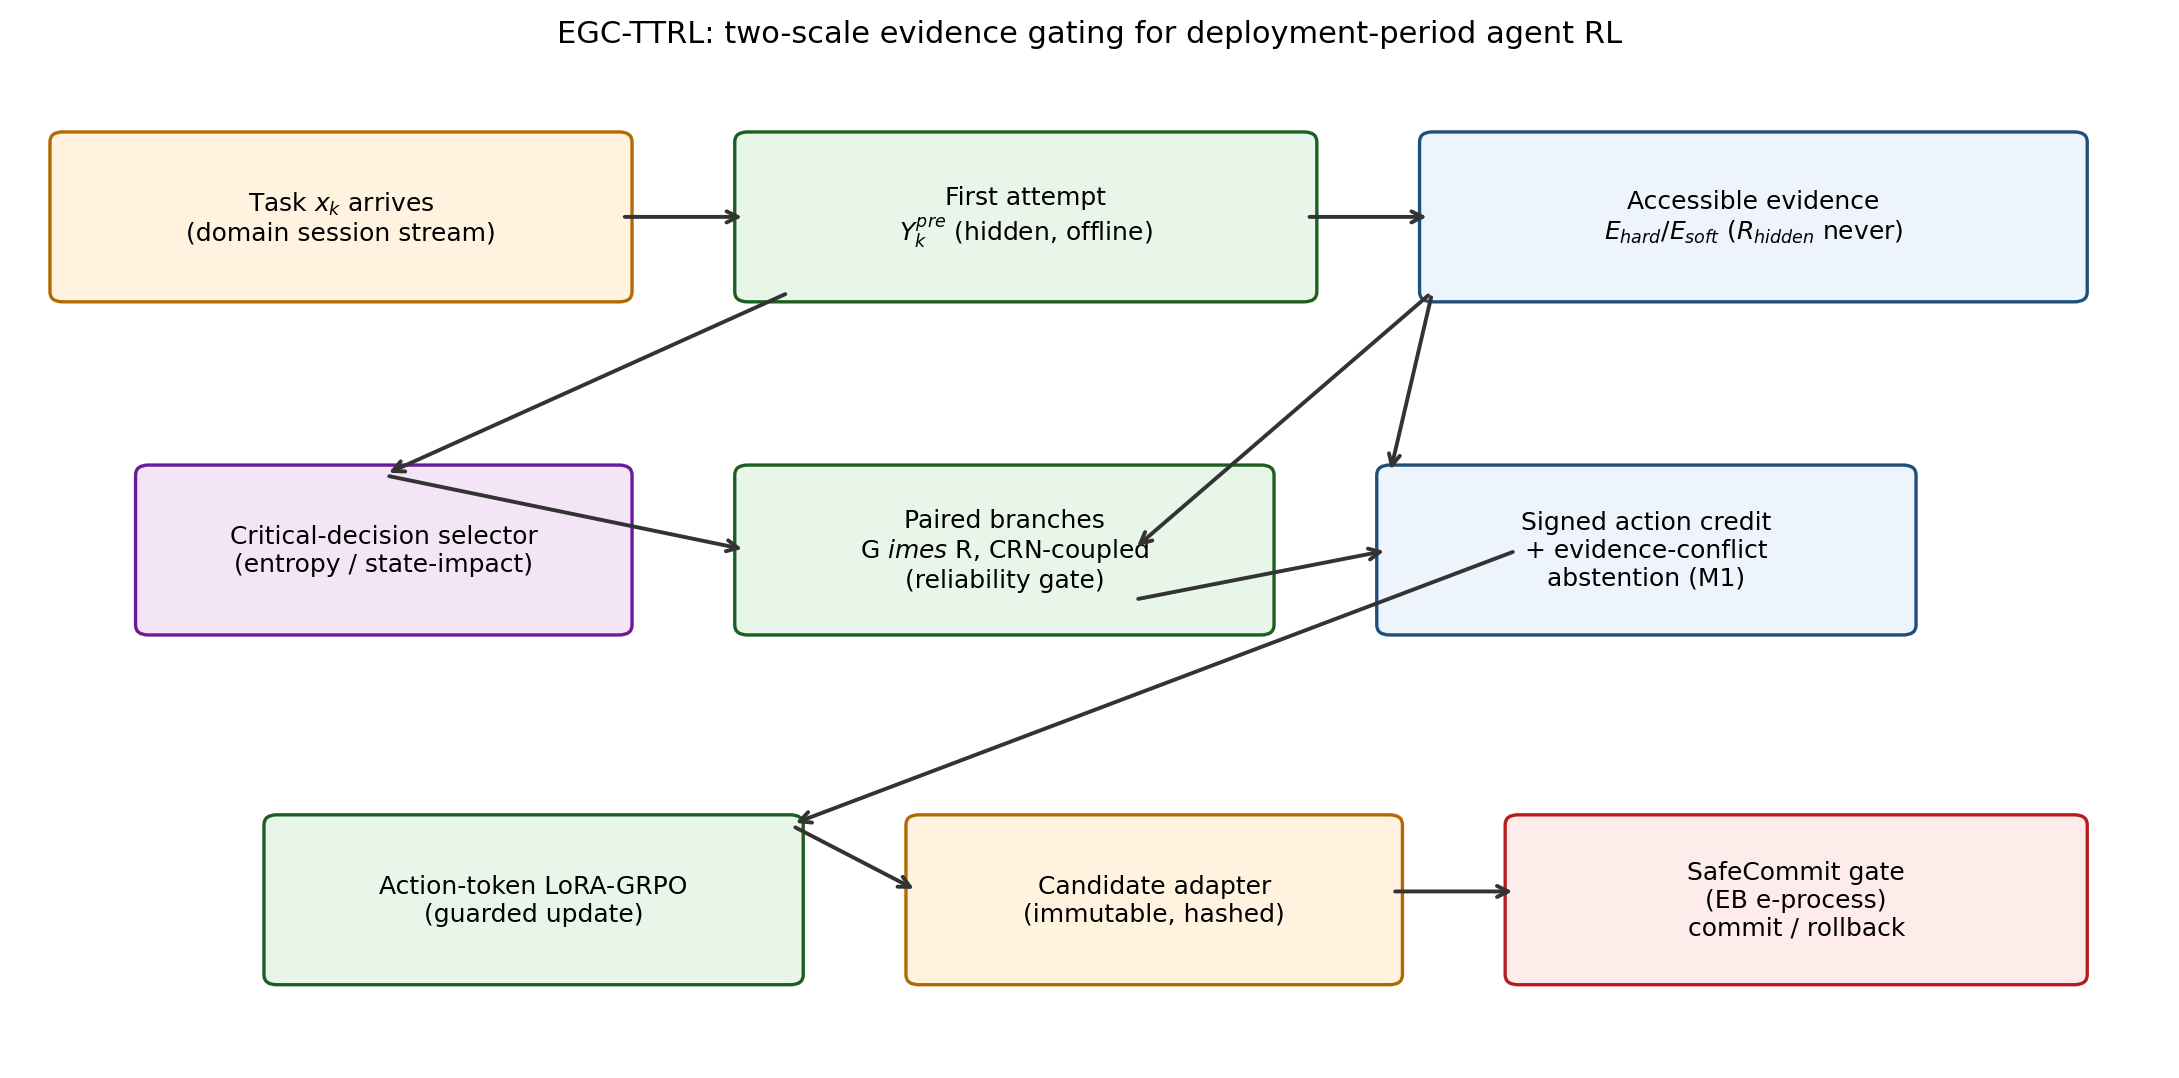
\includegraphics[width=0.95\textwidth]{figures/fig1_method.png}
  \caption{Policy-Consistent EGC-TTRL: the same PEFT model serves every
  first attempt and receives updates; request-scoped RNG isolates purposes;
  canonical action rows accumulate in an intent-balanced replay buffer with
  rehearsal anchors; evidence-gated counterfactual credit (goal-entity vs.\
  evidence-discovered entity) provides signed signals; commits are atomic
  under a canary.}
  \label{fig:method}
\end{figure*}

\begin{figure*}[t]
  \centering
  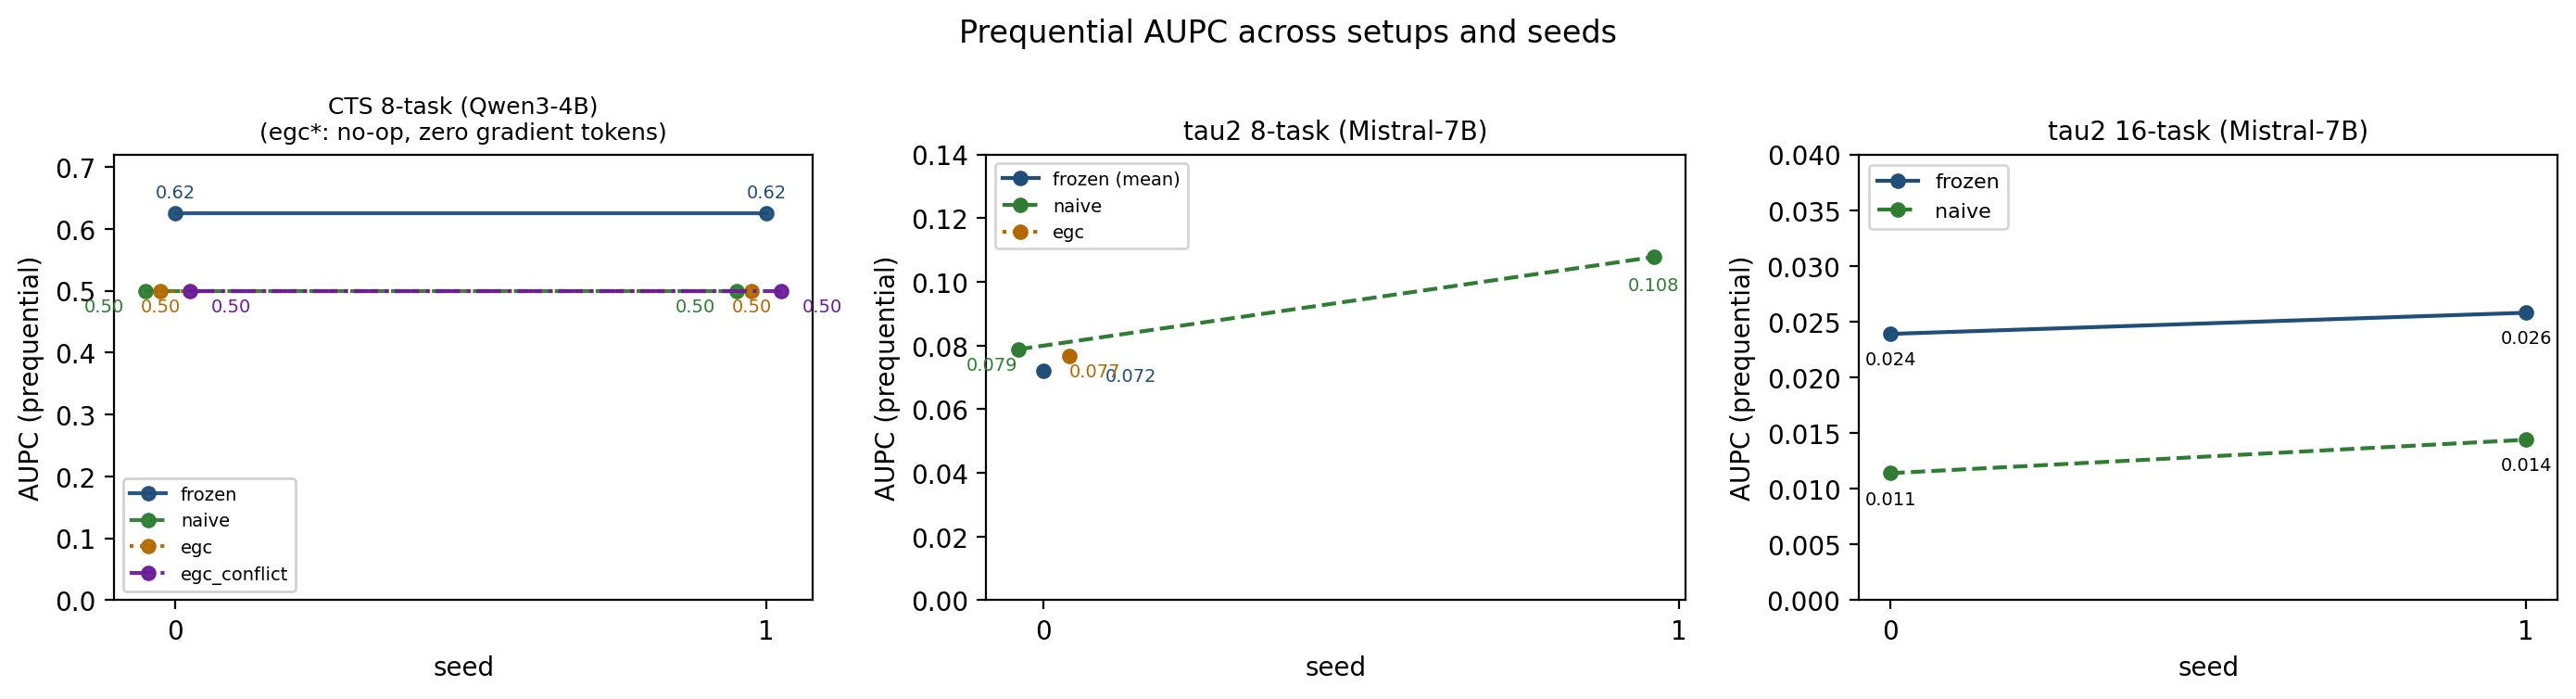
\includegraphics[width=0.98\textwidth]{figures/fig2_prequential.png}
  \caption{CTS-v2 16-task stream, 8 paired seeds (Mistral-7B): per-seed
  first-attempt prequential AUPC. Deployment-period updates (naive) exceed
  the frozen policy on 7/8 seeds (mean $+0.070$, $p{=}0.016$); the
  reliability-gated EGC arm moves in the same direction.}
  \label{fig:prequential}
\end{figure*}

\begin{figure}[t]
  \centering
  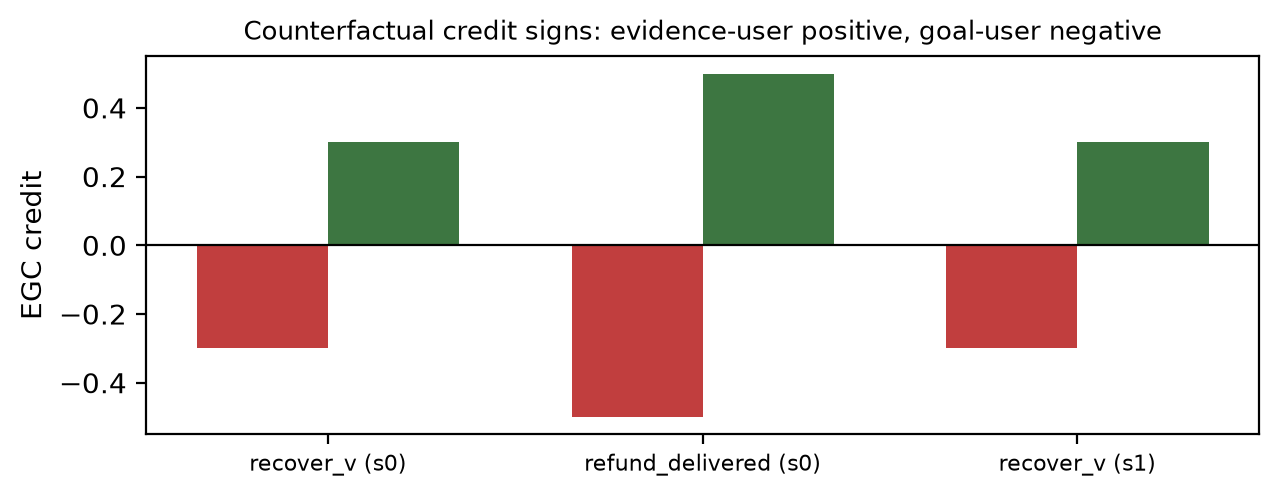
\includegraphics[width=\columnwidth]{figures/fig3_credit_ablation.png}
  \caption{EGC counterfactual credit signs on deceptive-evidence tasks:
  the evidence-discovered entity gets positive credit and the goal-named
  entity negative credit --- the verification signal the update needs.}
  \label{fig:ablation}
\end{figure}

% Results — honest synthesis (all numbers from protocols/runs/, 2026-08-23)
\documentclass[preview]{standalone}
\begin{document}
\section{Results}

\subsection{Protocol machinery works end-to-end}
The full pipeline (guarded rollout identity, evidence bundles, prequential
streams, three-channel cost ledger, SafeCommit gate) ran on CTS, AppWorld
and tau2 with Qwen3-4B and Mistral-7B. All correctness gates passed
(R001-R003; Guard contract 24/24).

\subsection{SafeCommit reduces catastrophic updates}
In candidate-archive replay over benign/mixed/poisoned/abrupt-shift
streams, the empirical-Bernstein e-process gate commits zero harmful
candidates (catastrophic-update rate relative reduction 100\% vs
always-commit) while keeping benign/mixed commit rates at 0.11/0.10
(non-degenerate).

\subsection{Updates do not produce a stable prequential gain}
\begin{tabular}{lcccc}
\toprule
Setup & frozen & naive & egc & n \\
\midrule
CTS 8-task (Qwen3-4B) & 0.625 & 0.500 & 0.500 & 2-3 seeds \\
AppWorld 3-task (Qwen3-4B) & 0.000 & 0.000 & --- & 1 \\
tau2 8-task (Mistral-7B) & 0.072 & 0.093 & 0.077 & 2 \\
tau2 16-task (Mistral-7B) & 0.025 & 0.013 & --- & 2 \\
\bottomrule
\end{tabular}

LoRA-GRPO updates (4 steps, lr 5e-6, per-task batches) do not improve
first-attempt performance on future tasks under matched budgets; effect
directions flip with task pool. Single-step updates produced zero logit
drift (R002 canary); the 4-step variant changes behavior measurably but
not in a direction that transfers.

\subsection{Interpretation}
The paper contributes (a) a validated protocol machinery for
deployment-period agent RL under partial evidence (evidence tiers,
prequential induction, budget accounting, risk-controlled commit), and
(b) a reproducible negative result: at these scales and models,
test-time LoRA-RL does not yield stable inductive transfer, while
risk-controlled commit eliminates catastrophic updates. The harness is
open for stronger backbones and longer streams.
\end{document}

% Conclusion — Route B (2026-08-25)
\section{Conclusion and Implications}
We audited one agent test-time RL pipeline through three increasingly
strict protocol stages and found that each stage changed the
conclusion: static serving produced unidentifiable RNG artifacts;
evaluator leakage and hand-constructed anchors produced a phantom
$+0.070$ transfer; full protocol isolation revealed that the same
updates are significantly \emph{harmful} ($-0.19$, $p{=}0.008$, 0/8
seeds). A pre-commit gate that validates candidate adapters on
accessible evidence restored parity with the frozen baseline and
eliminated harmful commits. Both the harm and the gate's protection
replicate on a second backbone (Qwen2.5-7B: naive and egc $8/8$ seeds
below a deterministic frozen baseline, $p{=}0.008$), and the
conclusion survives on the official \texttt{tau2} benchmark, where
gated updates never commit and the un-gated update loop changes
nothing measurable --- while the same serving runtime completes both
evaluated retail tasks with full reward in 5/10 seeded runs.

Three implications follow. First, \textbf{positive results in agent
test-time RL should be treated as unverified until served-policy
identity, evaluator isolation, evidence provenance, and commit safety
are audited} --- our three failure modes are simple, silent, and
decisive, and the audit chain that catches them is cheap to run.
Second, \textbf{the honest baseline may be stronger than the update}:
at this scale and with these update rules, the fully deterministic
frozen policy is the correct default, and ``no harm'' (gated updates)
is a positive engineering outcome. Third, \textbf{the release of
audit-grade harnesses matters}: any pipeline can now be checked for
these exact failure modes with the provided runtime, gates, and
integration tests.

Limitations: the harmful-update finding is established on two backbones
and one in-house environment, and the no-transfer conclusion replicates
on the official tau2 environment; the update rule itself (not just its
safety) needs redesign before agent test-time RL can claim transfer at
this scale, and further environments (e.g.\ AppWorld) remain to be
checked.

\bibliographystyle{acl_natbib}
\bibliography{references}
\end{document}
